Results here, in past tense.


\subsection{Visualising Sparse Pathways}
    \begin{figure}
        \begin{subfigure}{\linewidth}
            \centering
            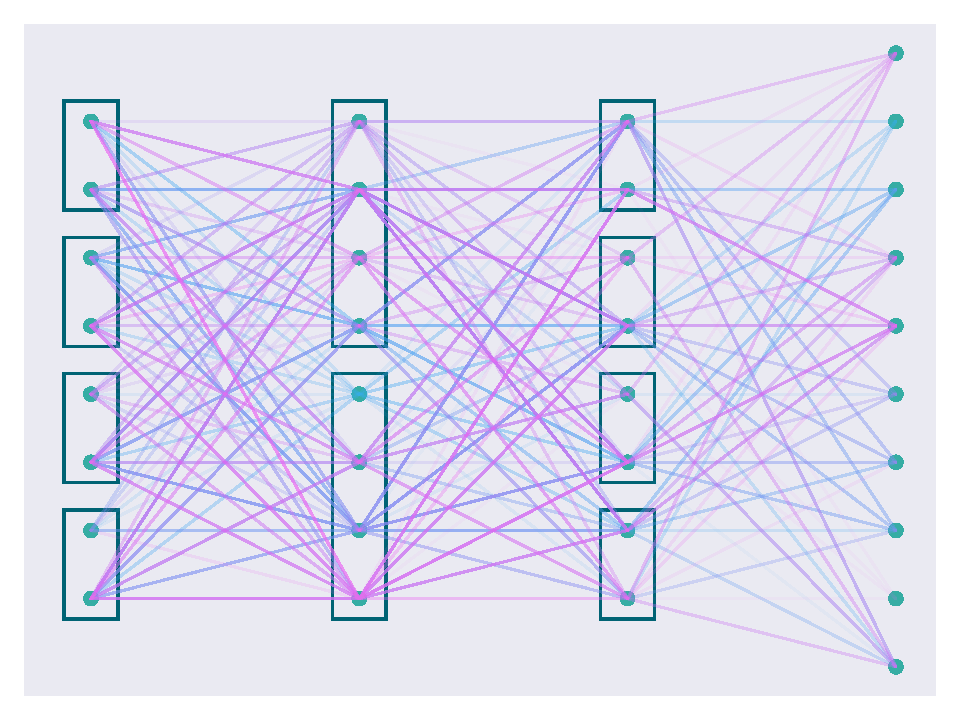
\includegraphics[width=\linewidth]{figs/LWTA_architecture_untrained.pdf}
            \caption{The untrained network predicting validation images of zeros in blue and ones in pink.}
            \label[fig]{LWTA_architecture_untrained}
        \end{subfigure}
        \begin{subfigure}{\linewidth}
            \centering
            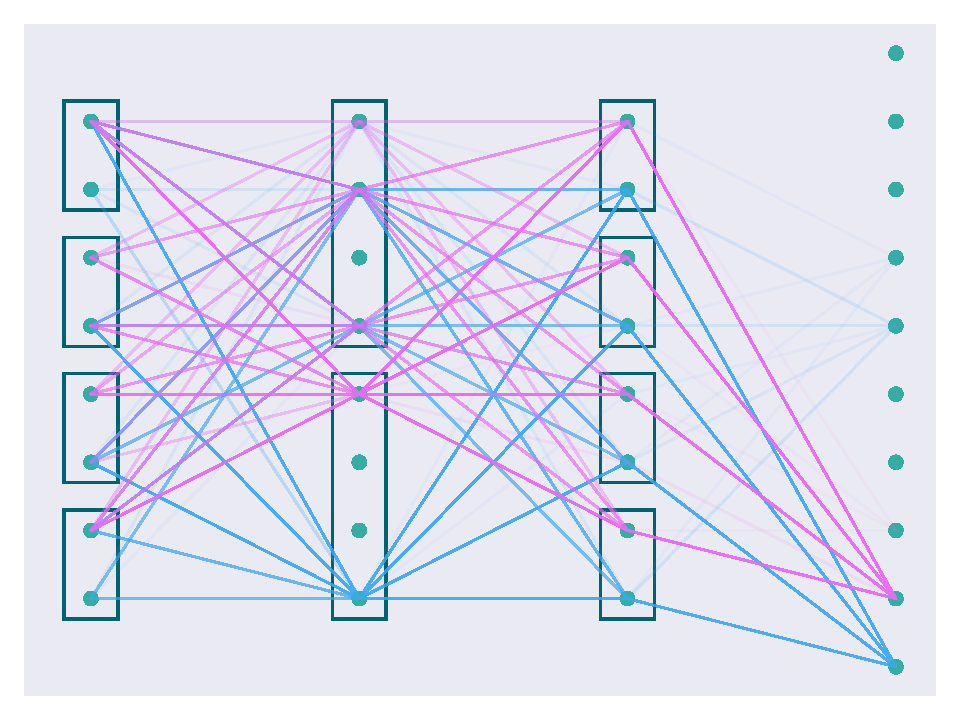
\includegraphics[width=\linewidth]{figs/LWTA_architecture_trained01.pdf}
            \caption{The trained network predicting validation images of zeros in blue and ones in pink.}
            \label[fig]{LWTA_architecture_trained01}
        \end{subfigure}
        \begin{subfigure}{\linewidth}
            \centering
            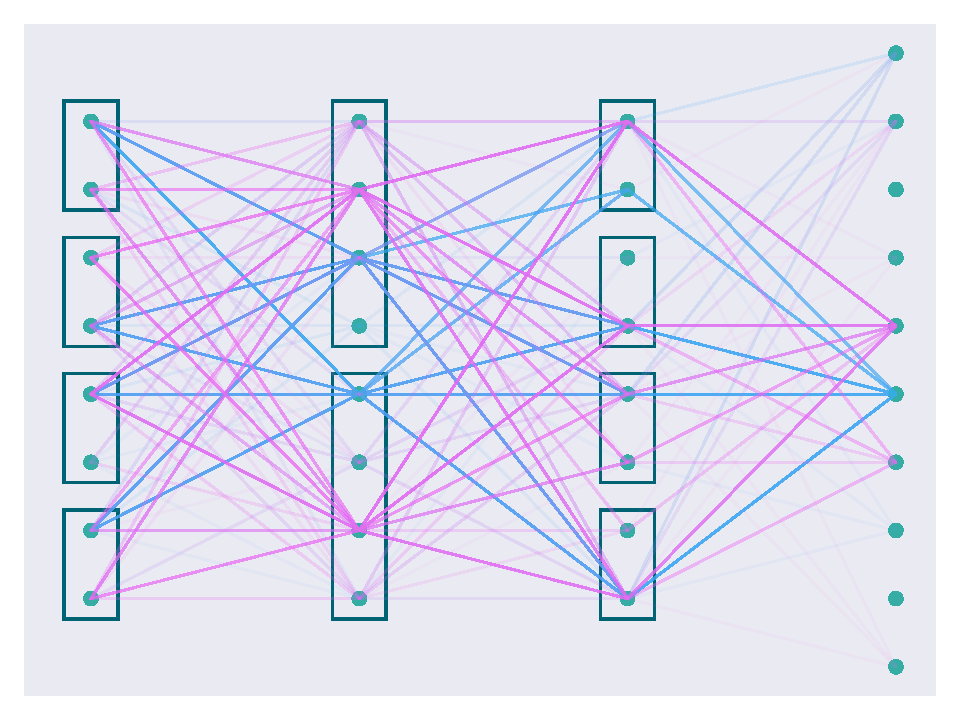
\includegraphics[width=\linewidth]{figs/LWTA_architecture_trained45.pdf}
            \caption{The untrained network predicting validation images of fours in blue and fives in pink.}
            \label[fig]{LWTA_architecture_trained45}
        \end{subfigure}
        \caption{An illustration of the active pathways as 100 input images belonging to two different classes are passed through a channel-out network. The network was trained on the full training dataset for 26 epochs before stopping early with $p=5$, and had a final validation accuracy of $0.8555$.}
        \label[fig]{LWTA_architecture}
    \end{figure}

\subsection{Tuning LWTA Architecture}
    \renewcommand{\arraystretch}{2}
    \begin{table}[ht!]
        \centering
        \begin{tabular}{|l|c|c|c|}
        \hline
        & \textbf{Regularisation} & \textbf{Architecture} & \textbf{Accuracy} \\
        \hline
        \rowcolor{mint!20}
        \cellcolor{mint!20} & None & \network{64, 32, 64}{32, 16, 8} & 0.4877 \\ \cline{2-4} 
        \rowcolor{mint!20}
        \cellcolor{mint!20} & Ridge & \network{64, 32}{32, *}  & 0.5090 \\ \cline{2-4} 
        \rowcolor{mint!50}
        \cellcolor{mint!20} & Dropout & \network{64, 64}{32, 16} & 0.5146 \\ \cline{2-4} 
        \rowcolor{mint!20}
        \multirow{-4}{*}{\rotatebox[origin=c]{90}{Maxout}}{\cellcolor{mint!20}} & Both & \network{32, 64}{16, 16} & 0.4943 \\ \hline
        \rowcolor{maroon!20}
        \cellcolor{maroon!20} & None & \network{64, 16, 32}{16, 8, *} & 0.4856 \\ \cline{2-4} 
        \rowcolor{maroon!50}
        \cellcolor{maroon!20} & Ridge & \network{64, 16, 64}{32, *, 32} & 0.5100 \\ \cline{2-4} 
        \rowcolor{maroon!20}
        \cellcolor{maroon!20} & Dropout & \network{32, 16, 64}{16, *, 32} & 0.4747 \\ \cline{2-4} 
        \rowcolor{maroon!20}
        \multirow{-4}{*}{\rotatebox[origin=c]{90}{Channel-Out}}{\cellcolor{maroon!20}} & Both & \network{32, 64}{16, 32} & 0.4917 \\ \hline
        \rowcolor{cyan!20} 
        \cellcolor{cyan!20} & None & \network{32,32}{} & 0.4843 \\ \cline{2-4} 
        \rowcolor{cyan!50} 
        \multirow{-2}{*}{\rotatebox[origin=c]{90}{Dense}}{\cellcolor{cyan!20} } & Ridge & \network{32,32}{} & 0.4899 \\ \hline
        \end{tabular}
        \caption{Table of }
        \label[tab]{res:tab:networks}
    \end{table}
    \renewcommand{\arraystretch}{1}
